





\section{Abstract}


\tmpsection{One or two sentences providing a basic introduction to the field}
% comprehensible to a scientist in any discipline.
\lettr{I}t is still unclear what factors determine the number of pathogens a wild species carries.
But once understood, these factors could provide a way to prioritise surveillance of wild populations for zoonotic disease and make predictions as to how pathogen richness will respond to global change.


\tmpsection{Two to three sentences of more detailed background}
% comprehensible to scientists in related disciplines.

% Theory led.

The pattern of contacts between individuals (i.e. population structure) has long been known to strongly affect epidemic processes.
Theory suggests that population structure can promote pathogen richness while the ecological literature generally assumes it will decrease richness.


\tmpsection{One sentence clearly stating the general problem (the gap)}
% being addressed by this particular study.

Previous studies in wild bat populations have had contradictory results and the different measures of population structure have different shortcomings.
There is therefore a need for more robust comparative studies testing for a relationship between pathogen richness and population structure.

\tmpsection{One sentence summarising the main result}
%  (with the words “here we show” or their equivalent).

Here I used comparative data to test whether population structure influences pathogen richness using bats as a case study as they have been associated with a number of important, recent zoonotic outbreaks.
Unlike previous studies I used two measures of population structure: a novel measure, number of subspecies, and a more careful application of genetic measures which have been used previously.
I find that both of these measures are positively associated with pathogen richness and are probably in the best supported model.


\tmpsection{Two or three sentences explaining what the main result reveals in direct comparison to what was thoughts to be the case previously}
% or how the main result adds to previous knowledge

My results add more robust support to the hypothesis that pathogen structure promotes pathogen richness in bats and lends clarity to the contradictory results previously published.
The results support predictions from theory.
They contradict the assumption commonly made in the ecological literature that factors that increase $R_0$ should increase pathogen richness implying that competitive processes amongst pathogens are stronger than previously thought.


\tmpsection{One or two sentences to put the results into a more general context.}

Although my analysis implies that population structure does promote pathogen richness in bats, the weakness of the relationship and the difficulty in obtaining some measurements means this is probably not a usefully predictive factor on it's own for optimising zoonotic surveillance.
However, the relationship has implications for global change, implying that increased habitat fragmentation might promote greater viral richness in bats.





%%%%%%%%%%%%%%%%%%%%%%%%%%%%%%%%%%%%%%%%%%%%%%%%%%%%%%%%%%%%%%%%%%%%%%%%%%%%%%%%%%%%%%%%%%%%%%%%%%%%%%%%%%%%%%%%%%%%%%%%%%%%%%%%%%%%%%%%%%%%%%%%%%%%%%%%%%%

\section{Introduction}

%%%%%%%%%%%%%%%%%%%%%%%%%%%%%%%%%%%%%%%%%%%%%%%%%%%%%%%%%%%%%%%%%%%%%%%%%%%%%%%%%%%%%%%%%%%%%%%%%%%%%%%%%%%%%%%%%%%%%%%%%%%%%%%%%%%%%%%%%%%%%%%%%%%%%%%%%%%

\tmpsection{General Intro}
The number of pathogen species carried by a host species has important consequences for the ecology of the host and the probability that the host will be a reservoir of a zoonotic pathogen.
However, the factors that affect pathogen richness are poorly understood.



\tmpsection{Specific Intro}



\tmpsection{Theoretical background}

%Think this ref is right but need to check.
Single pathogen models show that increasing population structure simply slows disease spread and makes establishment less likely \cite{colizza2007invasion, vespignani2008reaction}.
In the ecological literature this is often taken as predicting that increased population structure will decrease pathogen richness \cite{nunn2003comparative, morand2000wormy}.
However, models of competition between multiple pathogens show that in unstructured populations a competitive exclusion process occurs but that splitting the population into two patches allows coexistence \cite{qiu2013vector,allen2004sis, nunes2006localized}.


\tmpsection{Previous Studies}

Three studies have used comparative data to test for an association between population structure and viral richness.
A study on 15 African bats found a positive relationship between distribution fragmentation and viral richness \cite{maganga2014bat} while a study on 20 South-East Asian bats found the opposite relationship \cite{gay2014parasite}. 
A global study on 33 bats found a positive relationship between $F_{ST}$ --- a measure of genetic structure --- and viral richness \cite{turmelle2009correlates}. 
However, this study included measures using mtDNA which only measures female dispersal which may have biased the results many bat species show female philopatry \cite{kerth2002extreme, hulva2010mechanisms}.
Furthermore, this study used measures of $F_{ST}$ irrespective of the study scale with studies covering from tens \cite{mccracken1981social} to thousands \cite{petit1999male} of kilometers.
As isolation by distance has been shown in a number of bat species \cite{burland1999population, hulva2010mechanisms, o2015genetic, vonhof2015range} this could bias results further.
Finally, when a global $F_{ST}$ value is not given they used the mean of all pairwise $F_{ST}$ between sites.
This is not correct as from global $F_{ST}$ we expect migration rates of $M = (1-F_{ST})/8F_{ST}$ while from $F_{ST}$ between pairs of populations we expect migration rates of $M = (1-F_{ST})/16F_{ST}$ where $M$ is the absolute number of diploid inviduals dispersing per generation \cite{slatkin1995measure}.
To use studies that only present pairwise $F_{ST}$ values the raw data would have to be gathered and global $F_{ST}$ calculated from those.
As it is in fact the movement of individuals that is epidemiologically relavent, using these studies is probably not correct without attempting to correct for these difference.
Studies on single pathogens, notably rabies, have also shown that for virulent pathogens, space can allow persistence where a well mixed population ould experience a single, large epidemic then pathogen extinction \cite{blackwood2013resolving, pons2014insights}.


\tmpsection{Choice of measure of population structure}

A number of measurments of population structure have been used in the literature and each has it's own shortcomings.
In particular, the better, more direct measurements tend to be very work intensive which consequently means data is available for few species.

\tmpsection{Direct dispersal measurements}

The ideal metric of population structure is direct measurement of dispersal rates and distance.
These are incredibly difficult to obtain, especially over large scales.
Due to white nose syndrom, some very large mark-recapture studies have been conducted, but recapture rates are low \cite{}.
Further, these large studies have been in species that live in a few large colonies, so recapture rates should be higher than in less social species.
In practise, direct measurements are not practical for comparative analysis due to the lack of data and inconsistency in data collection methods.


\tmpsection{Genetic measures}

As direct measurement of dispersal are difficult, genetic data is often used.
Measurement such as $F_{ST}$ are used to calculate migration.
There are strong model assumptions under the conversion from $F_{ST}$ to migration.
However, the main issue with this measure is the effort required for each study and the subsequent low number of measurements.
Further, there are differences in the scales of the studies and the genetic regions being sequenced.
This differences should not be ignored.

\tmpsection{Number of Subspecies}

For a population to evolve distinct phenotypic or genetic traits, such that they can be classed as a subspecies, there must be limited migration between populations.
The number of subspecies a species has therefore reflects the level of population structure in that species.
The value of this measurement is available for every bat species.
However, it is likely biased, with well studied species being likely to have more recognised subspecies.
Further, this is a very course measure and it is important to consider whether it is measuring migration at a timescale and rate that is epidemiologically relevant.

For both measures from $F_{ST}$ and the number of subspecies it is useful to consider the rates of animal movement that are being measured.
Rates of migration estimated from $F_{ST}$ tend to be between 1 and 100 individuals per generation dispersing across all subpopulations.


\tmpsection{Measures from range}

The final measurement that has been used is derived from the shape of the species' range, typically from IUCN \cite{iucn} maps.
The ratio between the perimeter of the range and the area (or similar values) are calculated.
Range maps are very course for many species.
Furthermore there is a potential bias with island living species being given sea based edges where continental species might be assumed to live everywhere in between locations where it is known to live, without considering the different terrestrial habitats in these areas.

\tmpsection{The gap}

There is a lack of studies using multiple measures of population structure and larger datasets to robustly estimate the importance of population structure.


\tmpsection{What I did/found}

Here I have used two measures of population structure --- the number of subspecies and gene flow --- to robustly test for an association between population structure and pathogen richness in bats.
Furthermore, I used a much larger dataset for one of these analyses, further promoting robustness of results.
I found that both measures of population structure are positively associated with viral richness and are likely to be in the best models for describing viral richness.
Further, I found that the role of phylogeny is very weak in the models and in the distribution of viral richness amongst taxa.


%%%%%%%%%%%%%%%%%%%%%%%%%%%%%%%%%%%%%%%%%%%%%%%%%%%%%%%%%%%%%%%%%%%%%%%%%%%%%%%%%%%%%%%%%%%%%%%%%%%%%%%%%%%%%%%%%%%%%%%%%%%%%%%%%%%%%%%%%%%%%%%%%%%%%%%%%%%

\section{Methods}

%%%%%%%%%%%%%%%%%%%%%%%%%%%%%%%%%%%%%%%%%%%%%%%%%%%%%%%%%%%%%%%%%%%%%%%%%%%%%%%%%%%%%%%%%%%%%%%%%%%%%%%%%%%%%%%%%%%%%%%%%%%%%%%%%%%%%%%%%%%%%%%%%%%%%%%%%%%


























































To test for an association between pathogen richness I have performed multivariate regression using a model selection framework to establish whether or not two measures of pathogen richness are likely to be in a `best model' and therefore important.
As species cannot be considered independant due to shared evolutionary history, phylogeny was controlled for in all regressions.
A number of other factors that have previously been found to be important were included as additional independant variables (body mass \cite{kamiya2014determines, turmelle2009correlates, gay2014parasite, maganga2014bat}, range size \cite{kamiya2014determines, turmelle2009correlates, maganga2014bat} and study effort \cite{turmelle2009correlates, gay2014parasite, maganga2014bat}).
This was to attempt to avoid spurious positive results occuring simply due to correlation between pathogen richness and a different, causal factor.
Despite commonly bein associated with pathogen richness \cite{arneberg2002host, kamiya2014determines, nunn2003comparative}, population density is not included in the analysis as there is very little data for bat densities --- however Chapter 4 examines the relationship between density and population structure and Chapter 5 presents a method that allows the estimation of density from acoustic surveys.
I have both the number of subspecies a bat species has and estimates of gene flow (analysed separately) as measures of population structure.
All analyses were run in R \cite{R}

To measure pathogen richness I used data from \cite{luis2013comparison}. 
These simply include known infections of a bat species with a pathogen species. 
Only species with at least one pathogen were included in the analysis.
Rows with host species that were not identified to species level were removed.
Many viruses were not identified to species level or their identified species was not in the ICTV virus taxonomy \cite{ICTV}.
I counted a virus if it was the only virus, for that host species, in the lowest taxonomic level identified in the ICTV taxonomy.
That is, if a host carries an unknown Paramyxoviridae virus, then it must carry at least one Paramyxoviridae virus.
If a host carries an unknown Paramyxoviridae virus and a known Paramyxoviridae virus, then it is hard to confirm that the unknown virus is not another record of the known virus.
In this case, this would be counted as one virus species.






\begin{knitrout}\footnotesize
\definecolor{shadecolor}{rgb}{0.969, 0.969, 0.969}\color{fgcolor}\begin{figure}[t]

{\centering 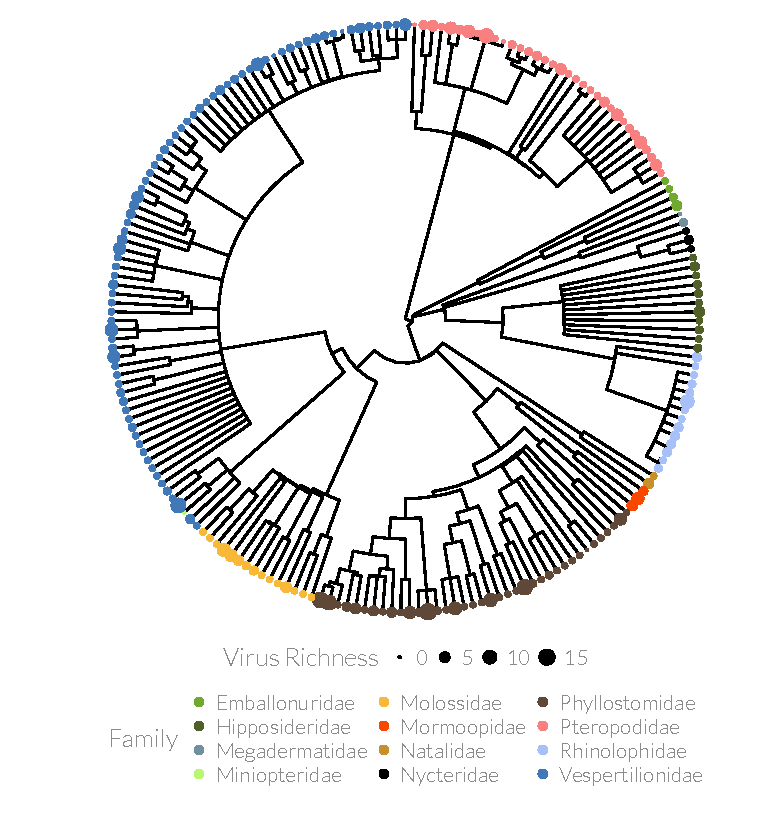
\includegraphics[width=\textwidth]{figure/treePlot-1} 

}

\caption[Pruned phylogeny with dot size showing number of pathogens and colour showing family]{Pruned phylogeny with dot size showing number of pathogens and colour showing family.}\label{fig:treePlot}
\end{figure}


\end{knitrout}










I used two measures of population structure. 
Gene flow and the number of subspecies.
The number of subspecies was counted using the Wilson and Reeder taxonomy \cite{wilson2005mammal}.
Gene flow is calculated from estimates of $F_{ST}$ collated from the literature.
Studies are from a wide range of spatial scales, from local ($\sim\SI{10}{\kilo\metre}$) to continental.
As $F_{ST}$ often increases with spatial scale \cite{burland1999population, hulva2010mechanisms, o2015genetic, vonhof2015range} I controlled for this by only using data from studies where a large proportion of the species range was studied.
I used the ratio of the furthest distance between $F_{ST}$ samples (measured with \url{http://www.distancefromto.net/} if not stated) to the width of the IUCN species range \cite{iucn} and only used studies if this ratio was greater than 0.2.
I converted all $F_{ST}$ value to migration using $M = \frac{1-F_{ST}}{8F_{ST}}$.
This removes the $(0, 1)$ bounds of $F_{ST}$ and is more easily interpretable though the results are unaffected. 
These two measures of population structure were analysed separately as the number of subspecies has 196 data points while there is only $F_{ST}$ data for 22 bat species.

To control for study bias I collected the number of Pubmed and Google Scholar citations for each bat species name including synonyms from ITIS \cite{itis} via the taxize package \cite{chamberlain2013taxize}.
The counts were scraped using the rvest package \cite{rvest}.
I log transformed these variables as they were strongly right skewed.
The log number of citations on Pubmed and Google scholar were highly correlated (pgls: $t$ = 19.32, df = 194, $p$ = 0).
As this corelation is strong, the results here are for analyses using only Google Scholar citations.
%See the appendix for analyses run using Pubmed citations.

Measures of body mass are taken from Pantheria \cite{jones2009pantheria} and primary literature \cite{canals2005relative, arita1993rarity, lopez2014echolocation, orr2013does, lim2001bat, aldridge1987turning, ma2003dietary, owen2003home, henderson2008movements, heaney2012nyctalus, oleksy2015high, zhang2009recent}. 
\emph{Pipistrellus pygmaeus} was assigned the same mass as \emph{P. pipistrellus} as they indistinguishable by mass.
Body mass measurements were log transformed due to the strong right skew.
Distribution size was estimated by downloading range maps for all species from IUCN \cite{iucn} and were also logged due to right skew.


To control for phylogenetic nonindependance I used the best-supported phylogeny from \textcite{fritz2009geographical} (shown in Figure~\ref{fig:treePlot}) which is the supertree from \cite{bininda2007delayed} with names updated to match the Wilson \& Reeder taxonomy \cite{wilson2005mammal}.
Phylogenetic manipulation was performed using the ape package \cite{ape}.
The importance of the phylogeny on each variable separately was estimated using \cite{caper}.
I also performed the analysis using the tree from \cite{jones2005bats} as this has some broad changes with families in different places.
However the phylogeny did not affect the analysis.







		
		























\begin{knitrout}\footnotesize
\definecolor{shadecolor}{rgb}{0.969, 0.969, 0.969}\color{fgcolor}\begin{figure}[t]

{\centering 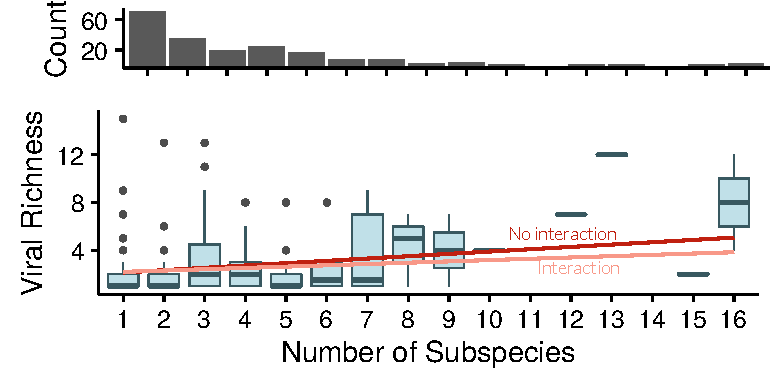
\includegraphics[width=0.8\textwidth]{figure/boxplot-1} 

}

\caption[Number of virus species against number of subspecies]{Number of virus species against number of subspecies. 		
The top panel shows the distribution of the data, with most species having few subspecies.		
Data within a number of subspecies are plotted as boxplots with the dark bar showing the median, the box showing the interquartile range, vertical lines showing the range and outliers shown as seperate points.		
Regression lines are from multivariate phylogenetic models with all other independant variables set at their median value.		
The models shown are those with (pink) and without (red) an interaction between study effort and number of subspecies.		
}\label{fig:boxplot}
\end{figure}


\end{knitrout}






%%%%%%%%%%%%%%%%%%%%%%%%%%%%%%%%%%%%%%%%%%%%%%%%%%%%%%%%%%%%%%%%%%%%%%%%%%%%%%%%%%%%%%%%%%%%%%%%%%%%%%%%%%%%%%%%%%%%%%%%%%%%%%%%%%%%%%%%%%%%%%%%%%%%%%%%%%%
%%%% FST ANALYSIS                                                                                                                                  %%%%%%%%
%%%%%%%%%%%%%%%%%%%%%%%%%%%%%%%%%%%%%%%%%%%%%%%%%%%%%%%%%%%%%%%%%%%%%%%%%%%%%%%%%%%%%%%%%%%%%%%%%%%%%%%%%%%%%%%%%%%%%%%%%%%%%%%%%%%%%%%%%%%%%%%%%%%%%%%%%%%
















%%begind.rcode

#### Read is full fstFinal dataframe

fstFinal <- read.csv('data/Chapter3/fstFinal.csv', row.names = 1)

%%end.rcode


































































